\chapter{Literature Review}
\label{chap:litreview}
\lhead{\emph{Literature Review}}
% \linespread{8}

% \doublespacing

\section{Introduction}



As we stand on the precipice of a future moulded by artificial intelligence and machine learning, one domain that is experiencing considerable progress is Optical Character Recognition (OCR). In this dynamic and continuously evolving field, there are many techniques which have emerged among the significant game-changers, two of these are the Tesseract OCR engine and Convolutional Recurrent Neural Networks (CRNNs). Tesseract, initially developed by Hewlett-Packard and later adopted by Google, is a pioneering engine that converts images of text into machine-encoded text, offering utilities across numerous applications. On the other hand, CRNNs, a deep learning-based approach, combine the spatial feature extraction capabilities of Convolutional Neural Networks (CNNs) with the sequential data processing capacity of Recurrent Neural Networks (RNNs). These networks have set new benchmarks in the realm of scene text recognition, overcoming the challenges posed by variations in text sizes, fonts, and orientations. This literature review delves into the intricacies of these advanced tools, shedding light on their principles, applications, strengths, and potential areas for improvement, thereby enriching our understanding of current trends in OCR technology and pointing to the future possibilities.


% In addition to these techniques, the selection of the correct font for each sensor is another critical element that affects the accuracy of the OCR system. Despite its importance, this aspect has been less emphasized in existing literature, thereby forming a crucial area of exploration in this study

This literature review explores the current state of OCR technologies, with a particular focus on Tesseract and CRNN models. It delves into various image pre-processing techniques, emphasizing the unique method of red and green colour masking before conversion to grayscale. Lastly, it investigates the role of font selection in enhancing OCR accuracy, thereby setting the context for the subsequent research.

While this review focuses on the capabilities of Tesseract OCR and Convolutional Recurrent Neural Networks (CRNNs) in the OCR domain, it's important to acknowledge that the OCR landscape is not limited to these technologies. Many other methods play equally significant roles in expanding the OCR frontiers and opening up new avenues for research and application. Long Short-Term Memory Networks (LSTMs), Transformers, attention-based OCR models, rule-based systems, Support Vector Machines (SVMs), Hidden Markov Models (HMMs), K-Nearest Neighbours (KNN), and template matching are some of these diverse methodologies that provide unique perspectives and solutions in the OCR realm. Each of these methods has its distinctive advantages, making them optimal for certain types of tasks, as well as its limitations, requiring continuous research and development for enhancement. However, the scope of this review will mainly revolve around Tesseract and CRNNs, while the mentioned methods provide an essential context for understanding the broader OCR ecosystem.

\newpage

\section{Tesseract OCR}

Optical character recognition (OCR) is the process of converting images of text into machine-readable text. Tesseract is an open-source Optical Character Recognition (OCR) engine that is widely used for a variety of tasks, including document digitization, machine translation, and data entry. Tesseract was developed at HP between 1984 and 1994. Initially conceived as a PhD research project to improve OCR performance for HP's scanners, it outperformed contemporary commercial OCR engines but never became an HP product. Its development was mainly focused on improving rejection efficiency rather than base-level accuracy. Despite being shelved in 1994, Tesseract proved its prowess in the 1995 UNLV Annual Test of OCR Accuracy. HP made Tesseract open-source in 2005, hosted at Google Code. Tesseract's architecture assumes binary images as input and uses a step-by-step pipeline for processing, including a unique connected component analysis for detecting inverse text. Its recognition process is two-pass: initial recognition of words feeds an adaptive classifier which subsequently improves text recognition further down the page. A final phase resolves fuzzy spaces and checks alternative hypotheses for the x-height to locate small-cap text. \cite{smithOverviewTesseractOCR2007}


\vspace{1cm}

\begin{figure}[ht]
    \centering
    
\includegraphics[width=0.6\textwidth]{Figures/tesseract_ocr.jpg}
    \caption[Tesseract OCR]{Tesseract OCR}\cite{liTrOCRTransformerBasedOptical2023}
    \label{fig:Tesseract OCR}
\end{figure}


In this literature review, we will discuss five research papers that have been published on Tesseract OCR. These papers cover a wide range of topics, including the accuracy of Tesseract, the performance of Tesseract on different types of documents, and the use of Tesseract for specific applications. Each study presents unique findings, and together they create a comprehensive overview of the current state and potential trajectory of Tesseract OCR. Through a detailed exploration of these works, we aim not only to comprehend the nuances of Tesseract OCR but also to contribute to the burgeoning discourse around its implications and opportunities in our increasingly digitized world

In the paper "Benchmarking Object Detection Algorithms for Optical Character Recognition of Odometer Mileage" Andersson et al. compare two state-of-the-art object detection models, Faster R-CNN and YOLO, with an open-source OCR model, Tesseract, for reading the odometer mileage from car dashboard images. They use a dataset of 2,389 images of car odometers and evaluate the models based on mean average precision, prediction accuracy, and Levenshtein distance.

\begin{figure}[ht]
    \centering
    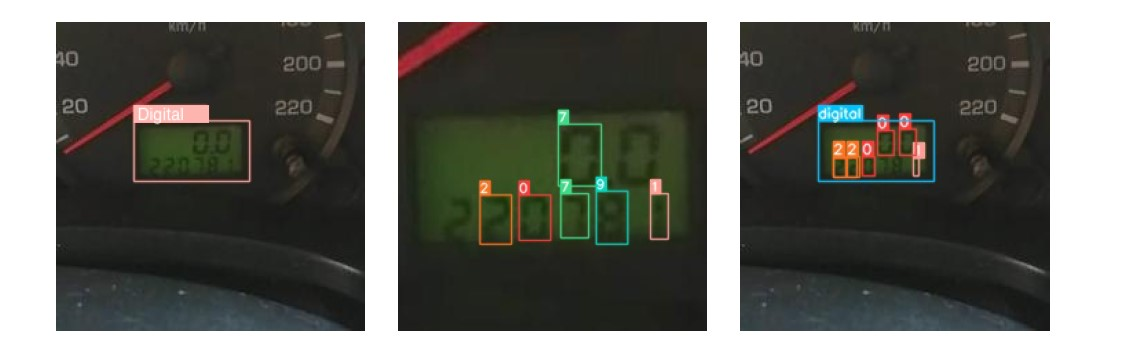
\includegraphics[width=0.88\textwidth]{Figures/tesseract_papers/Andersson_2022.jpg}
    \caption[Visualization of Boundary box predictions, and digit classification from
        YOLO-models. left - YOLO Singlebox-model. middle - YOLO Digitbox-model. right - YOLO
        Multibox-model.]{Visualization of Boundary box predictions, and digit classification from
        YOLO-models. left - YOLO Singlebox-model. middle - YOLO Digitbox-model. right - YOLO
        Multibox-model.}\cite{anderssonBenchmarkingObjectDetection2022}
    \label{fig:Andersson Visualisation of Boundary box predictions}
\end{figure}


They find that the object detection models outperform Tesseract on all metrics, and that Faster R-CNN has the highest mAP and accuracy, while YOLO has the lowest Levenshtein distance. \cite{anderssonBenchmarkingObjectDetection2022}


Ahuja et al.'s paper "Detecting Vehicle Type and License Plate Number of different Vehicles on Images" discusses the development of a model that can locate a particular vehicle that the user is looking for depending on two factors 1. the Type of vehicle and the 2. License plate number of the car. The proposed system uses a unique mixture consisting of Mask R-CNN model for vehicle type detection, WpodNet and Tesseract for License Plate detection and Prediction of letters in it.
\cite{ahujaDetectingVehicleType}

\begin{figure}[ht]
    \centering
    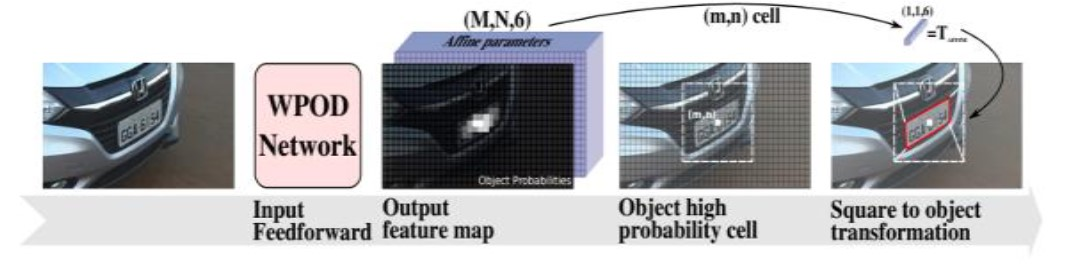
\includegraphics[width=0.88\textwidth]{Figures/tesseract_papers/Ahuja_2021.jpg}
    \caption[WpodNet Detection Method]{WpodNet Detection Method}\cite{ahujaDetectingVehicleType}
    \label{fig:WpodNet Detection Method}
\end{figure}

The first stage of Ahuja et al.'s project involved annotating 2,650 images with a custom dataset using the open-source tool VGG Annotator. The images were annotated with rectangular shapes instead of polygons, and the categories were 2-Wheelers, 3-Wheelers, 4-Wheelers, and vehicles with more than four wheels. The trained Mask R-CNN model achieved an F1 score of 0.72399 on the training data and 0.68 on the test data.

The second stage was split into two parts: license plate detection and letter classification. The WpodNet model was used for license plate detection, achieving an accuracy rate of over 90\%. The Tesseract model was then used to predict the letters on the license plate, enhancing speed and accuracy.

The third and final stage of the project involved the model accepting user input for vehicle type, license plate, and image. The model then compared this input with its output to determine if the searched vehicle had been identified.

The final hybrid model uses Mask R-CNN (F1 score: 0.72399 training, 0.68 testing), WpodNet, and pytesseract for car and license plate identification. This can aid in tracking stolen vehicles and assessing parking lot availability.


In an interesting paper, Giridhar et al.'s "A Novel Approach to OCR using Image Recognition based Classification for Ancient Tamil Inscriptions in Temples" describes a novel approach to OCR using image recognition based classification for ancient Tamil inscriptions in temples. The proposed work focuses on improving optical character recognition techniques for ancient Tamil script which was in use between the 7th and 12th centuries. A data set has been curated using cropped images of characters found on certain temple inscriptions, specific to this time period as a case study.

\begin{figure}[ht]
    \centering
    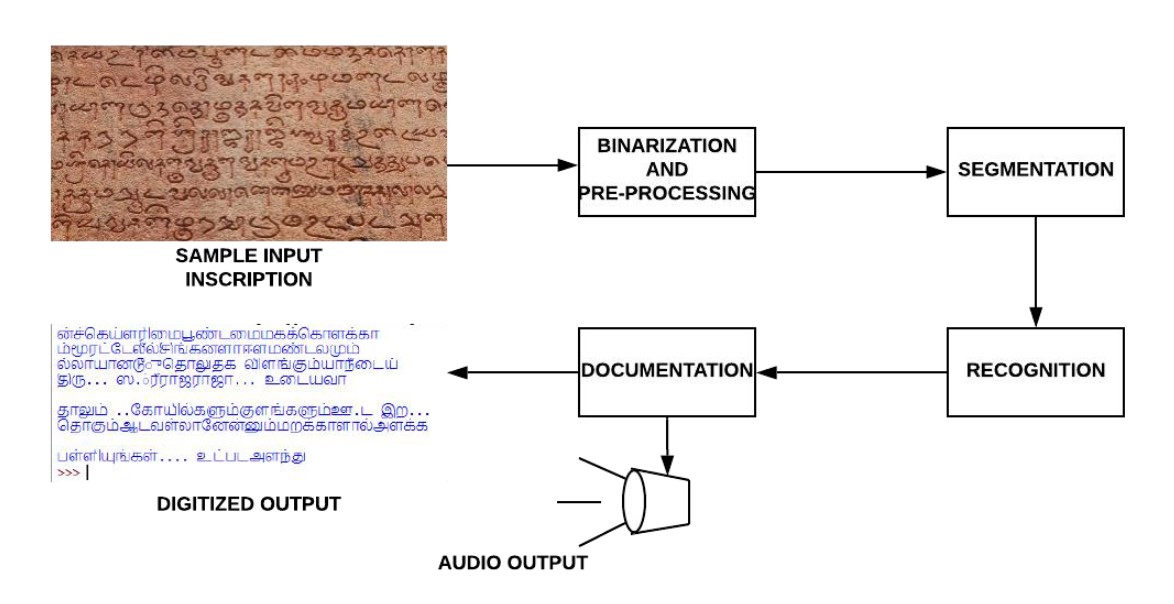
\includegraphics[width=0.88\textwidth]{Figures/tesseract_papers/Giridhar_2019.jpg}
    \caption[Giridhar's proposed architecture]{Giridhar's proposed architecture}\cite{giridharNovelApproachOCR2019}
    \label{fig:Giridhar's proposed architecture}
\end{figure}


After using Otsu thresholding method for binarization of the image, a two-dimensional convolution neural network is defined and used to train, classify, and recognize the ancient Tamil characters. To implement the optical character recognition techniques, the neural network is linked to the Tesseract using the Pytesseract library in Python. As an added feature, this work also incorporates Google's text to speech voice engine to produce an audio output of the digitized text. Various samples for both modern and ancient Tamil were collected and passed through the system.


The author used Otsu Thresholding Method for binarization of the image and a Two-dimensional Convolution Neural Network to train, classify, and recognize the ancient Tamil characters. To implement the optical character recognition techniques, the neural network is linked to the Tesseract using the Pytesseract library in Python. As an added feature, this work also incorporates Google's text to speech voice engine to produce an audio output of the digitized text.

On average, the combined efficiency of the system for ancient Tamil script was 77.7\%, although it varied based on the specific challenges encountered with different types of text and inscriptions. The study acknowledged that further work is needed to overcome these issues and increase the system's accuracy and efficiency.\cite{giridharNovelApproachOCR2019}

In Cakic et al's paper "The Use of Tesseract OCR Number Recognition for Food Tracking and Tracing", they discuss the use of computer vision and optical character recognition (OCR) on mobile devices to read serial numbers from wine labels in order to enable applications based on tracking and tracing of each individual wine bottle. The research focuses on the implementation and image processing that improved detection accuracy.

\begin{figure}[ht]
    \centering
    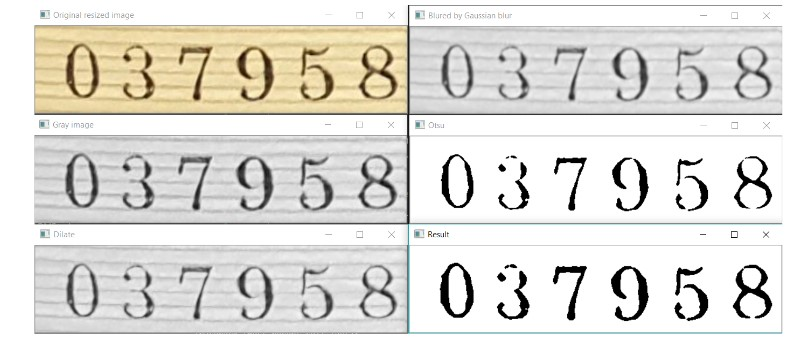
\includegraphics[width=0.88\textwidth]{Figures/tesseract_papers/Cakic_2020.jpg}
    \caption[Numbers change through the pre-processing stage]{Numbers change through the pre-processing stage}\cite{cakicUseTesseractOCR2020}
    \label{fig:Cakic's Numbers change through the preprocessing stage}
\end{figure}

Cakic et al.'s research involved testing a script to read serial numbers from about 150 wine label images, some of which were of poor quality. The initial attempt, which didn't involve any image pre-processing, managed to correctly read the full serial numbers on around 62\% of the images. After pre-processing the images, the success rate increased significantly to 87.5\%. This suggests that the quality of the pre-processing and the images used in the test dataset significantly affects the accuracy of the results.

In 2019, Robby et al.'s paper "Implementation of Optical Character Recognition using Tesseract with the Javanese Script Target in Android Application" discusses the challenges and methods of recognising non-Latin scripts, especially Javanese, which have complex shapes and structures. They present their dataset collection, training, and testing process using Tesseract OCR tools. They report their results and analysis, showing that their model achieved the highest accuracy by combining single boundary box and separate boundary boxes for different parts of the characters.

\begin{figure}[ht]
    \centering
    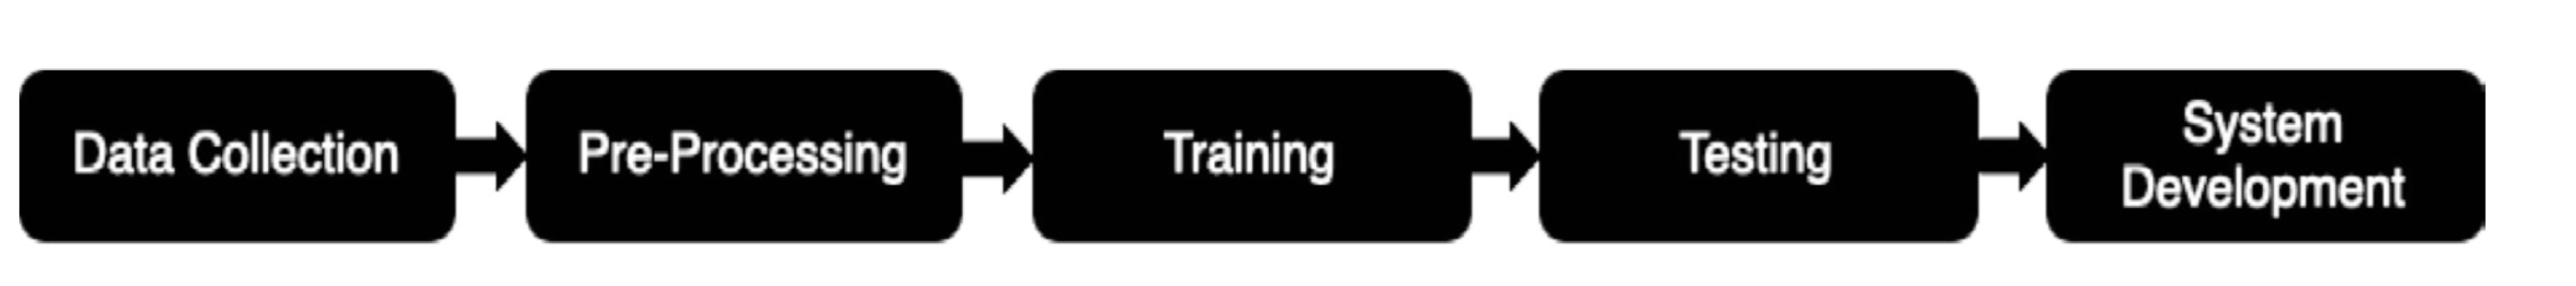
\includegraphics[width=0.88\textwidth]{Figures/tesseract_papers/Robby_2019.jpg}
    \caption[Robby et al.'s Proposed Method]{Robby et al.'s Proposed Method}\cite{robbyImplementationOpticalCharacter2019}
    \label{fig:Robby et al.'s Proposed Method}
\end{figure}


The authors of this paper used a variety of methods to develop a Javanese character recognition system. First, they collected 5880 Javanese characters from various sources and cropped and resized them to 32x32 pixels. Then, they applied several pre-processing steps to the images, such as binarization, noise removal, contrast enhancement, and skew correction. Next, they augmented the data by applying random rotations, translations, scaling, and shearing to the images. Finally, they used Tesseract, an open source OCR tool, to train different models with different boundary box methods.

The author's found that the best model was the one that combined single boundary box and separate boundary boxes for different parts of the characters, which achieved an accuracy of 97.50\% and an error rate of 2.50\% on the test set.


\newpage
\section{Convolutional Recurrent Neural Networks (CRNNs)}

CRNN, an abbreviation for Convolutional Recurrent Neural Network, is a unique fusion of the advantages of convolutional neural networks (CNN) and recurrent neural networks (RNN), which are different kinds of neural network architectures.

CRNNs are usually applied in the classification and analysis of sequential data like text, speech, and images. Due to their ability to handle variable-length sequential data and recognize long-term dependencies, they are extremely useful for tasks that need to comprehend contextual and temporal information. They have displayed excellence in modelling and processing sequential data across diverse tasks, marking them as an efficient instrument in this domain.\cite{vermaImprovementOCRTechnologies2022}

\subsection{Working of CRNNs}
The functionality of CRNNs is outlined as follows:

\begin{enumerate}
    \item \textbf{Input:} The primary input to a CRNN is a sequence of data, which could be images or audio samples.
    \item \textbf{Convolutional Layers:} The incoming sequence is channelled through convolutional layers, akin to those in CNNs. These layers extract features from the input and are particularly efficient for image-based inputs.
    \item \textbf{Recurrent Layers:} The output from a convolutional layer is then sent through one or more recurrent layers. These layers preserve a hidden state that memorizes information from previous entries in the sequence, making them ideal for sequential data processing.
    \item \textbf{Bridge between Convolutional and Recurrent Layers:} Usually, the output from a convolutional layer is sampled before it is introduced to a recurrent layer. This strategy helps to minimize the network's computational complexity while maintaining the core characteristics of the input.
    \item \textbf{Output:} Finally, the output from the last recurrent layer is processed through a fully connected layer. This final layer produces a prediction for the input sequence, which could be a string of characters, words, or any other output related to the task.
\end{enumerate}

In the article "Synthetized Multilanguage OCR Using CRNN and SVTR Models for Realtime Collaborative Tools" Biro et al. present a novel hybrid language vocabulary creation method that is utilized in the OCR training process in combination with convolutional recurrent neural networks (CRNNs) and a single visual model for scene text recognition within the patch-wise image tokenization framework (SVTR). The research used a dedicated Python-based data generator built on dedicated collaborative tool-based templates to cover and simulate the real-life variances of remote diagnosis and co-working collaborative sessions with high accuracy. The machine learning models recognized the multilanguage/hybrid texts with high accuracy.

\begin{figure}[ht]
    \centering
    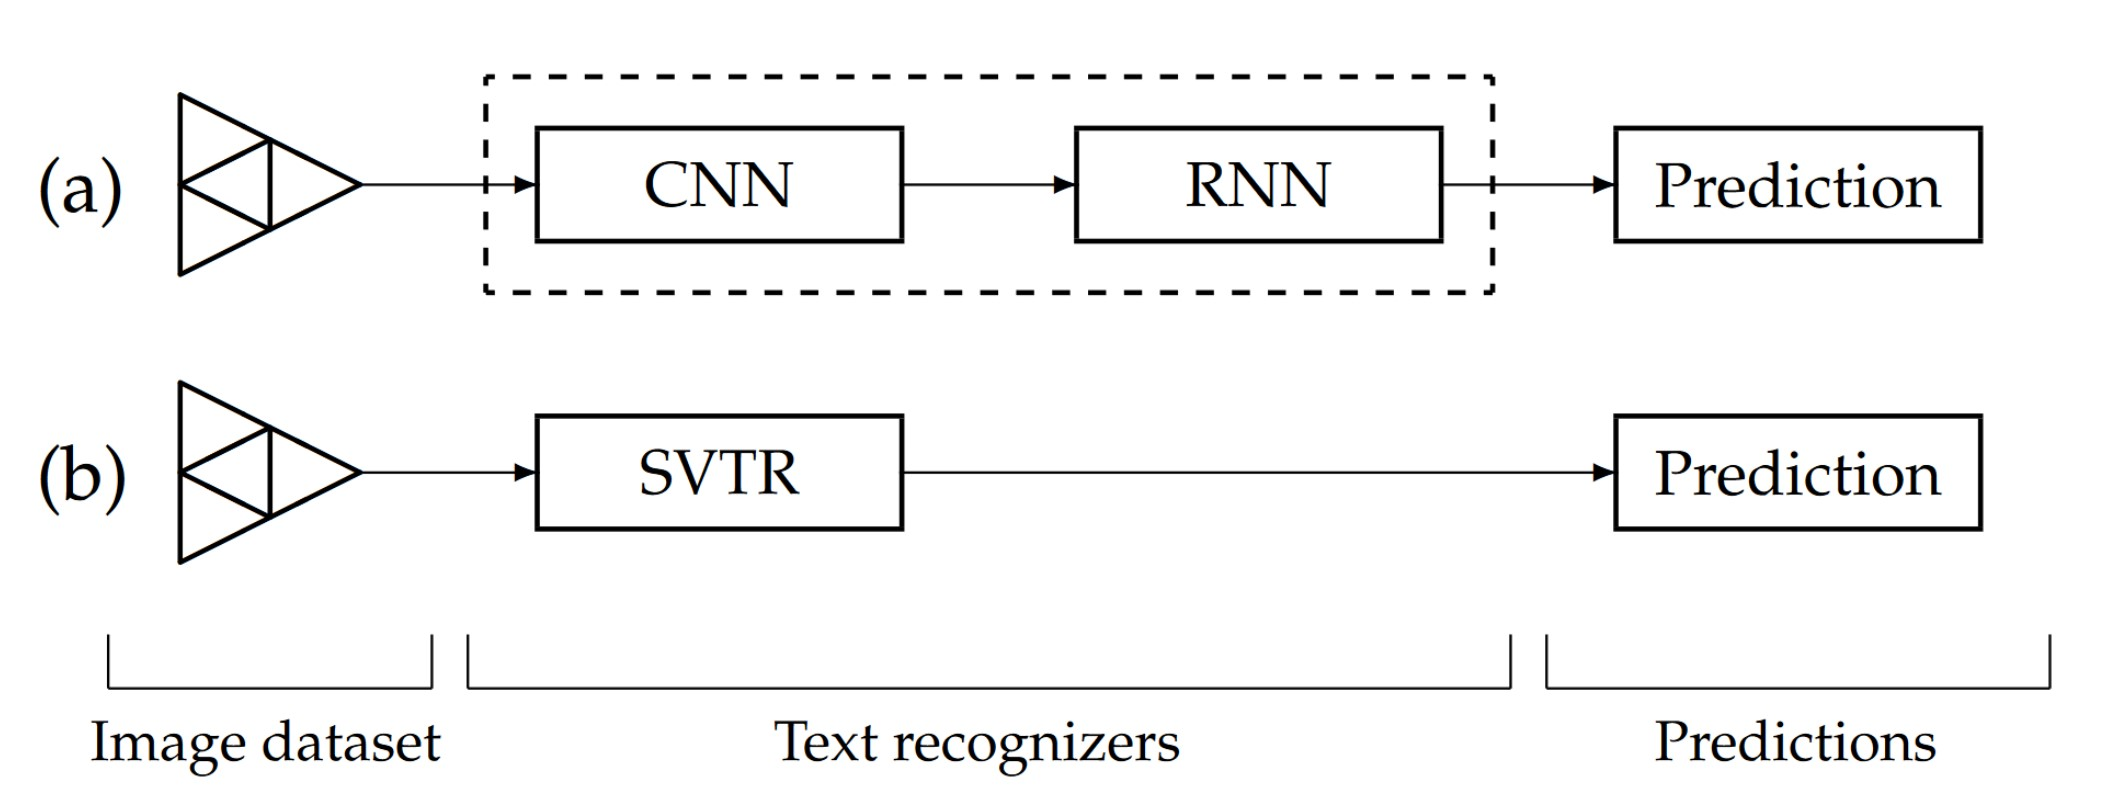
\includegraphics[width=0.88\textwidth]{Figures/CRNN_Papers/Biro_2023.jpg}
    \caption[Biro et al.'s Modern Recogniser]{Biro et al.'s Modern text recognizers using (a) CRNN and (b) SVTR models}\cite{biroSynthetizedMultilanguageOCR2023}
    \label{fig:Biro et al.'s Modern text recognizers using CRNN and SVTR models}
\end{figure}


The highest precision scores achieved are 90.25\%, 91.35\%, and 93.89\%. The study examines the feasibility of machine learning-supported OCR in a multilingual environment. The novelty of our method is that it provides a solution not only for different speaking languages but also for a mixture of technological languages, using artificially created vocabulary and a custom training data generation approach. The machine learning models for special multilingual, including languages with artificially made vocabulary, perform consistently with high accuracy. \cite{biroSynthetizedMultilanguageOCR2023}



Shinde et al.'s paper "Using CRNN to Perform OCR over Forms"  presents a structured process of locating input fields on the form, scanning the input data, processing the data and entering the data to the final database. The methods used in this system is a general method of performing OCR on human handwriting. The form filled by the user is to be scanned and sent as an input to the system. The model will then detect all the user input areas on the form as the main goal is to extract the user-entered information only. The system architecture consists of a Word Segmentation algorithm followed by a neural network architecture to perform optical character recognition on the words after segmenting them from the sentences. The convolutional layers are used to extract feature sequences from the input images. This output is passed on to the recurrent layers for making predictions for each frame of the feature sequence. Finally, the transcription layer or the CTC is used to translate the per-frame predictions by the recurrent layers into a label sequence.

\begin{figure}[ht]
    \centering
    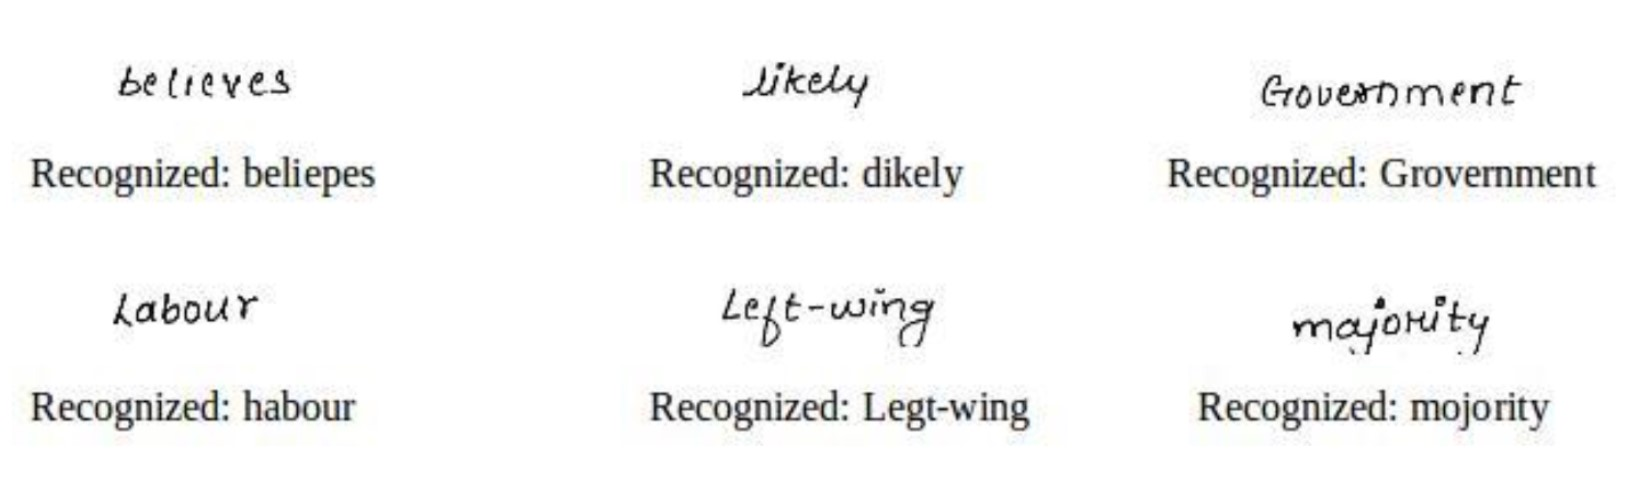
\includegraphics[width=0.88\textwidth]{Figures/CRNN_Papers/Shinde_2020.jpg}
    \caption[Shinde et al.'s Handwriting Results]{Shinde et al.'s Handwriting Results}\cite{shindeUsingCRNNPerform2021}
    \label{fig:Shinde et al.'s Handwriting Results}
\end{figure}

The study found that handwriting styles that matched those of the IAM dataset (which feature larger spaces between words and smaller spaces within words) were correctly segmented and recognized. However, when users wrote words closely together (congested handwriting), the system had trouble distinguishing between words, as the spacing between words was similar to the spacing between letters.

The increased inter-word spacing improved the accuracy of word segmentation and recognition. After testing the system with 100 random words, it achieved an accuracy of 72.22\%. Some errors were noted. For instance, the system mistook the letter "l" for "d" and "a" for "o". This suggests the system struggles with closely resembling words and varied handwriting styles.

The document proposes solutions to improve system accuracy, such as training the model on a wider variety of handwriting styles beyond those in the IAM dataset. Also, it suggests increasing the number of words in the training set relevant to the problem statement, like station names or sequences of numbers similar to mobile numbers, to enhance the probability of correct recognition.\cite{shindeUsingCRNNPerform2021}


In 2018, Rawl et al.'s paper "How To Efficiently Increase Resolution in Neural OCR Models" discusses how modern CRNN OCR models require a fixed line height for all images. Increasing this input resolution improves recognition performance up to a point. However, doing so by simply increasing the line height of input images without changing the CRNN architecture has a large cost in memory and computation. The authors introduce a few very small convolutional and max pooling layers to a CRNN model to rapidly down sample high resolution images to a more manageable resolution before passing off to the "base" CRNN model. Doing this greatly improves recognition performance with a very modest increase in computation and memory requirements.

\begin{figure}[ht]
    \centering
    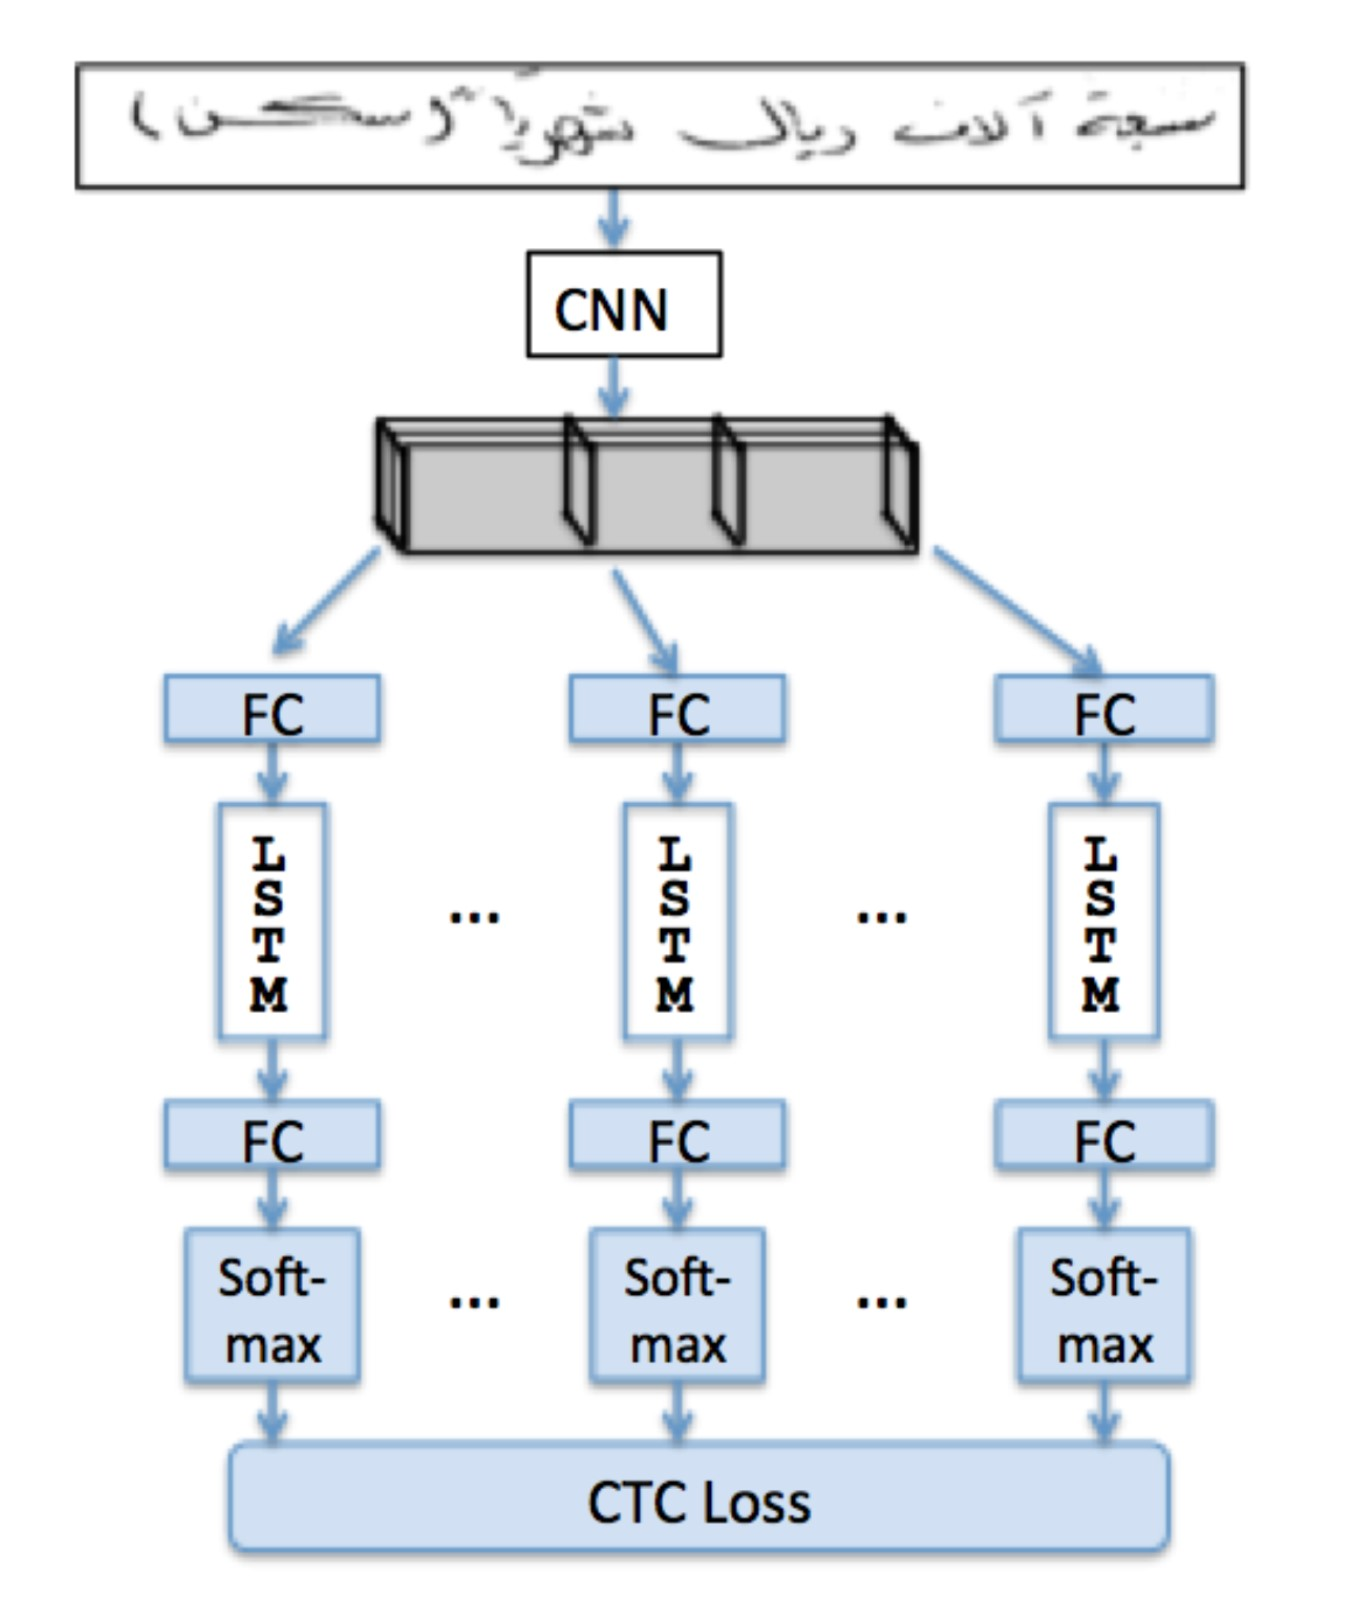
\includegraphics[width=0.58\textwidth]{Figures/CRNN_Papers/Rawl_2018.jpg}
    \caption[Rawl et al.'s End-to-End OCR Model: With CNN and LSTM layers]{Rawl et al.'s End-to-End OCR Model: With CNN and LSTM layers}\cite{rawlsHowEfficientlyIncrease2018}
    \label{fig:Rawl et al.'s End-to-End OCR Model: With CNN and LSTM layers}
\end{figure}


They show a 33\% relative improvement in WER, from 8.8\% to 5.9\% when increasing the input resolution from 30px line height to 240px line height on OpenHART/MADCAT Arabic handwriting data. The authors report new state-of-the-art results for both Arabic handwriting recognition and English handwriting recognition. They do this by increasing the resolution of input images from a line height of 30px to 240px, an 8-fold increase.\cite{rawlsHowEfficientlyIncrease2018}


In Wuhan, Feng et al.'s paper "Port Container Number Recognition System Based on Improved YOLO and CRNN Algorithm" discusses the deep learning-based container number recognition system. The system is composed of two parts: object detection and character recognition. The system is designed to recognize container numbers from images captured in real-world scenarios.


\begin{figure}[ht]
    \centering
    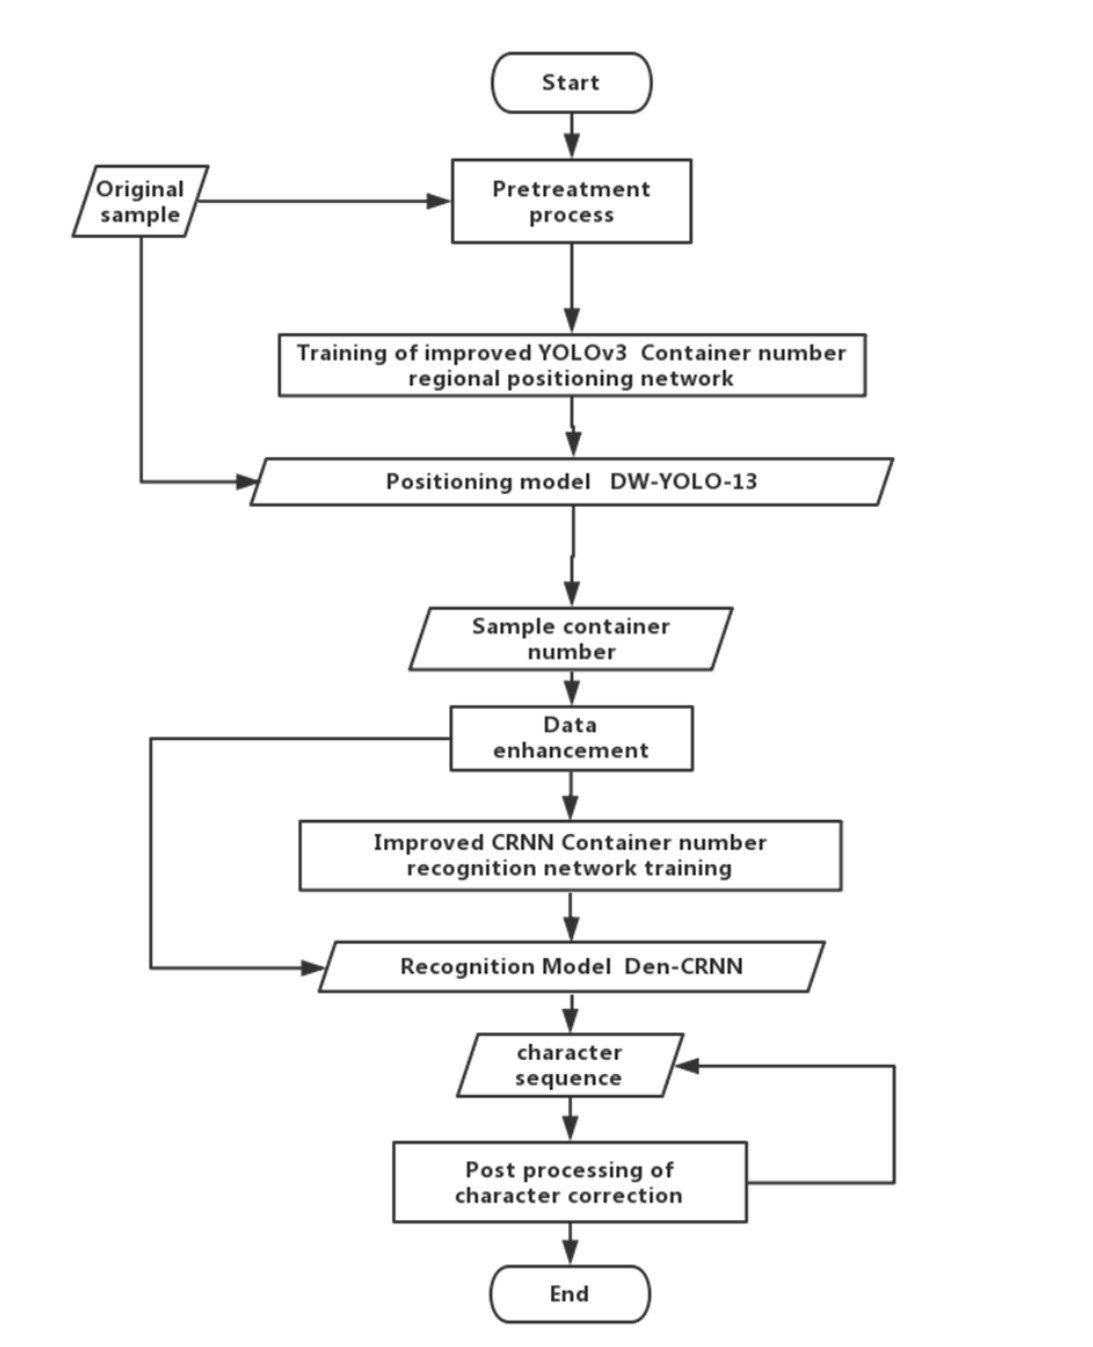
\includegraphics[width=0.58\textwidth]{Figures/CRNN_Papers/Feng_2020.jpg}
    \caption[Feng et al.'s Algorithm Structure]{Feng et al.'s Algorithm Structure}\cite{fengPortContainerNumber2020}
    \label{fig:Feng et al.'s Algorithm Structure}
\end{figure}

The object detection part uses YOLOv3 to detect the container number region and the character recognition part uses CRNN to recognize the characters in the region.  The system was tested on a dataset of 2000 images and achieved an accuracy of 98.5\%.\cite{fengPortContainerNumber2020}



In the paper "MultiPath ViT OCR: A Lightweight Visual Transformer-based License Plate Optical Character Recognition" by Azadbakht et al. present a new approach to OCR of license plates using a lightweight model based on Visual Transformer architecture. The proposed model is lightweight and can be used on edge devices with limited computation power.


\begin{figure}[ht]
    \centering
    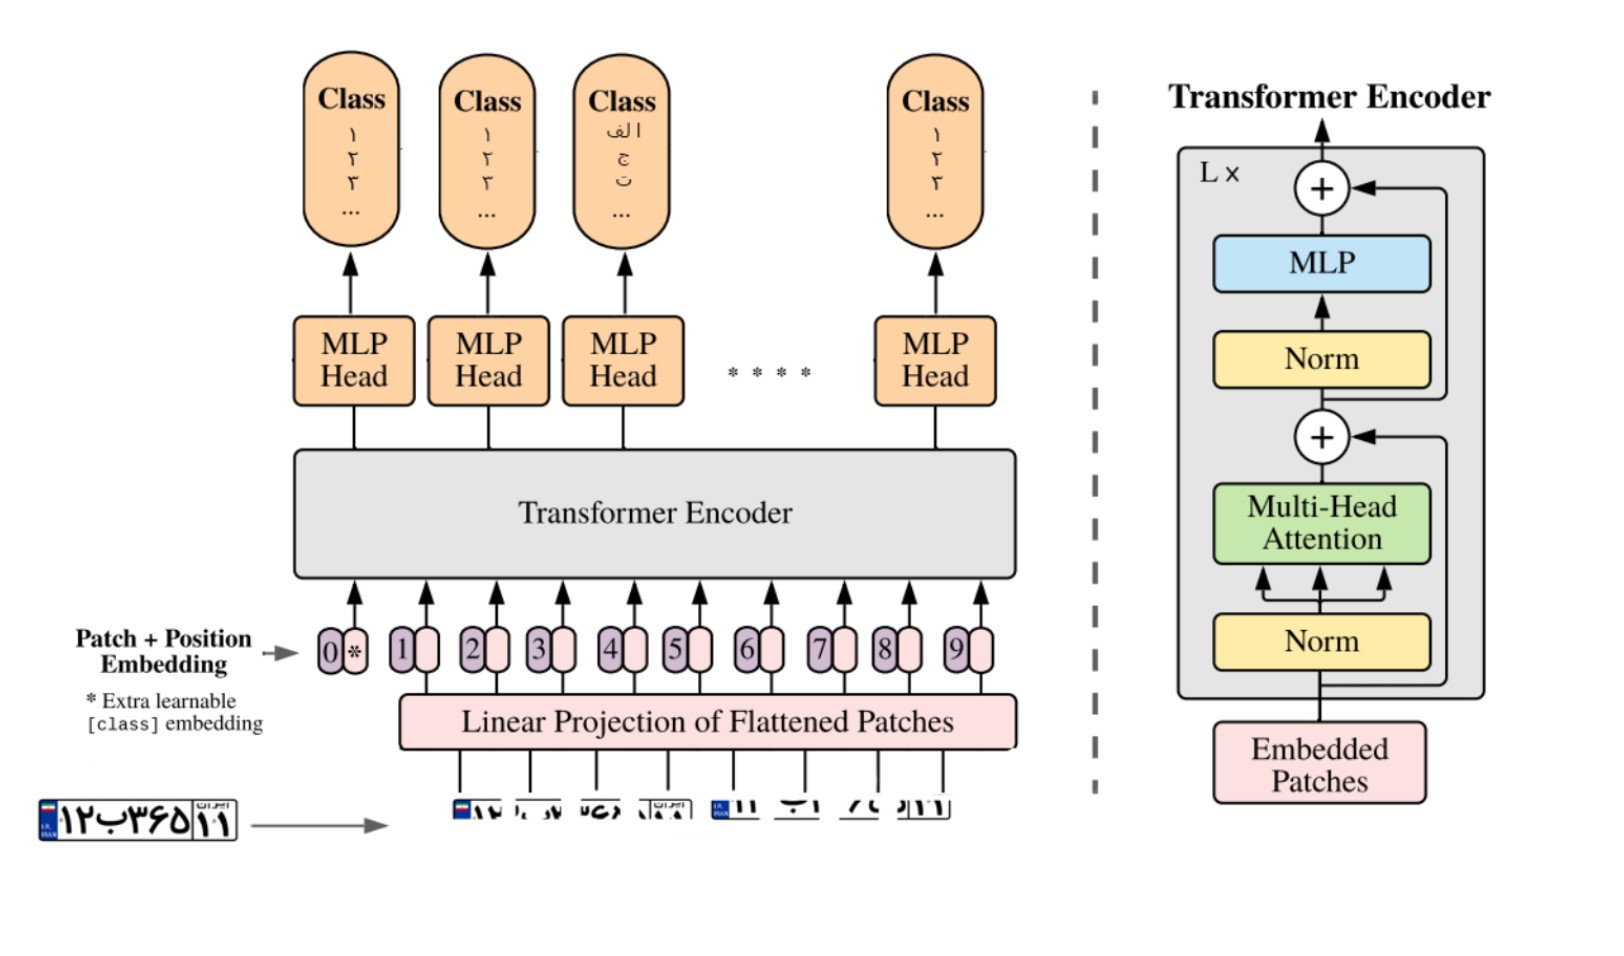
\includegraphics[width=0.78\textwidth]{Figures/CRNN_Papers/Azadbakht_2022.jpg}
    \caption[Azadbakht et al.'s MultiPath Visual Transformer OCR architecture]{Azadbakht et al.'s MultiPath Visual Transformer OCR architecture}\cite{azadbakhtMultiPathViTOCR2022}
    \label{fig:Azadbakht et al.'s MultiPath Visual Transformer OCR architecture}
\end{figure}

It achieves 77.25\% accuracy against CNN models with 75.18\% accuracy and embedded OCR models in cameras with 60.37\% accuracy on the LicenseNet test set. The authors gathered and annotated 1.3M images of license plates in various natural conditions from different points of view and different cameras and call this dataset as LicenseNet. The proposed model has 3.21 times fewer training parameters than previously proposed CNN-based models and achieves better accuracy with fewer parameters. The paper also explains the implementation details and training hyperparameters and compares the model's performance against the previously employed models.\cite{azadbakhtMultiPathViTOCR2022}

\newpage

\section{Other OCR Methods}

\subsection{Long Short-Term Memory Networks (LSTMs)}

Long Short-Term Memory Networks (LSTMs) are a special kind of recurrent neural network capable of learning long-term dependencies, which makes them highly suitable for OCR tasks. They've been used successfully to decode sequences of characters from images.\cite{breuelHighPerformanceOCRPrinted2013}

Breuel et al. in the paper "High-Performance OCR for Printed English and Fraktur using LSTM Networks" write about a novel application of bidirectional Long Short-Term Memory (LSTM) networks to the problem of machine-printed Latin and Fraktur recognition, without segmentation, language modelling or post-processing.

\begin{figure}[ht]
    \centering
    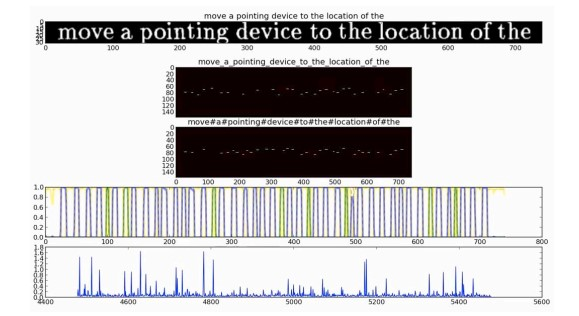
\includegraphics[width=0.8\textwidth]{Figures/LSTM_Breuel.jpg}
    \caption[Bruel's illustration of the training steps of the LSTM recognizer]{Greyscale image with background cleaning}\cite{breuelHighPerformanceOCRPrinted2013}
    \label{fig:Breuel LSTM Paper}
\end{figure}



A pre-processing step for text-line normalisation that uses a dictionary of connected component shapes and associated baseline and x-height information to map the input text lines to a fixed size output image.

A comparison of the LSTM-based system with other OCR systems on printed English and Fraktur texts, showing that LSTM achieves very low error rates and generalizes well to unseen data.

\newpage

\subsection{Transformers}

Originally developed for natural language processing tasks, Transformer models have been adapted for OCR. They treat the OCR problem as a sequence-to-sequence translation task, translating the input image into a sequence of characters.

\begin{figure}[ht]
    \centering
    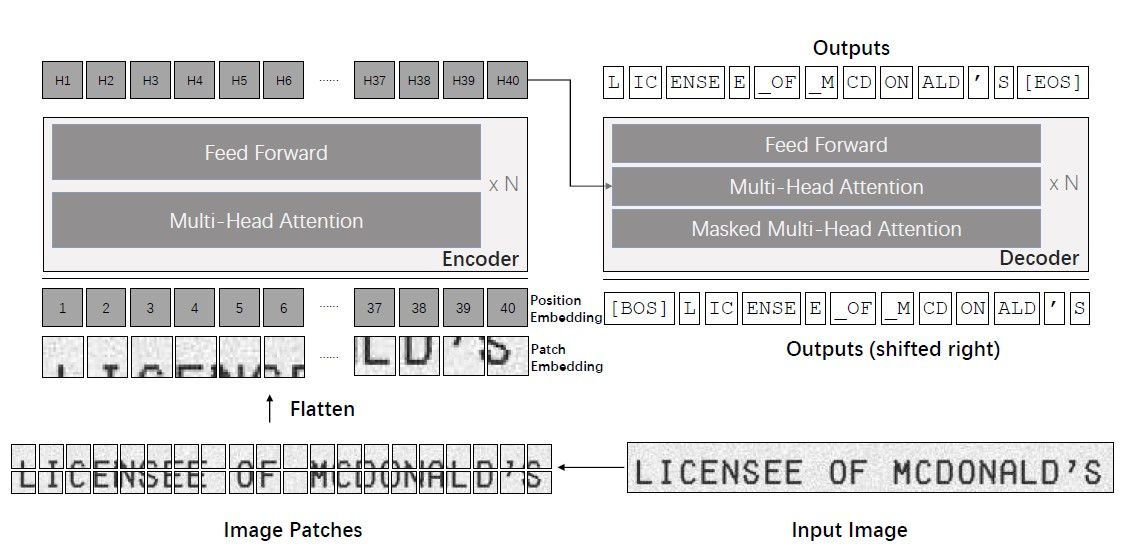
\includegraphics[width=0.6\textwidth]{Figures/Trans_MLi.jpg}
    \caption[Li's Architecture of TrOCR]{Li's Architecture of TrOCR}\cite{liTrOCRTransformerBasedOptical2023}
    \label{fig:Li's Architecture of TrOCR}
\end{figure}

M.Li et al.'s "TrOCR: Transformer-Based Optical Character Recognition with Pre-trained Models" paper proposes an end-to-end text recognition approach with pre-trained image Transformer and text Transformer models, which leverages the Transformer architecture for both image understanding and word piece-level text generation. \cite{liTrOCRTransformerBasedOptical2023}

Transformer based OCR models have the advantage of being able to handle long sequences of text, which is useful for OCR tasks. However, they are computationally expensive and require large amounts of training data.

CRNNs are more suitable for this project because they are faster and require less training data and are better at handling spatial information

\newpage

\subsection{Attention-based OCR models}

Attention mechanisms allow models to focus on different parts of the input image while predicting each character in the output sequence, similar to how humans read. This can improve accuracy, especially on more complex images.

Li et al.'s "Attention Based RNN Model for Document Image Quality Assessment" paper proposes a novel method for document image quality assessment (DIQA). The method integrates convolutional neural networks (CNNs) and recurrent neural networks (RNNs) to capture spatial features and attention mechanisms. It also uses reinforcement learning to train a locator network that selects the optimal regions for quality evaluation.

The CNNs are used to extract spatial features from the document images. The RNNs are used to capture the temporal dependencies between the features. The locator network is used to select the optimal regions for quality evaluation. The regions are selected based on the attention mechanism, which identifies the most important regions in the document images. \cite{liAttentionBasedRNN2017}


\begin{figure}[ht]
    \centering
    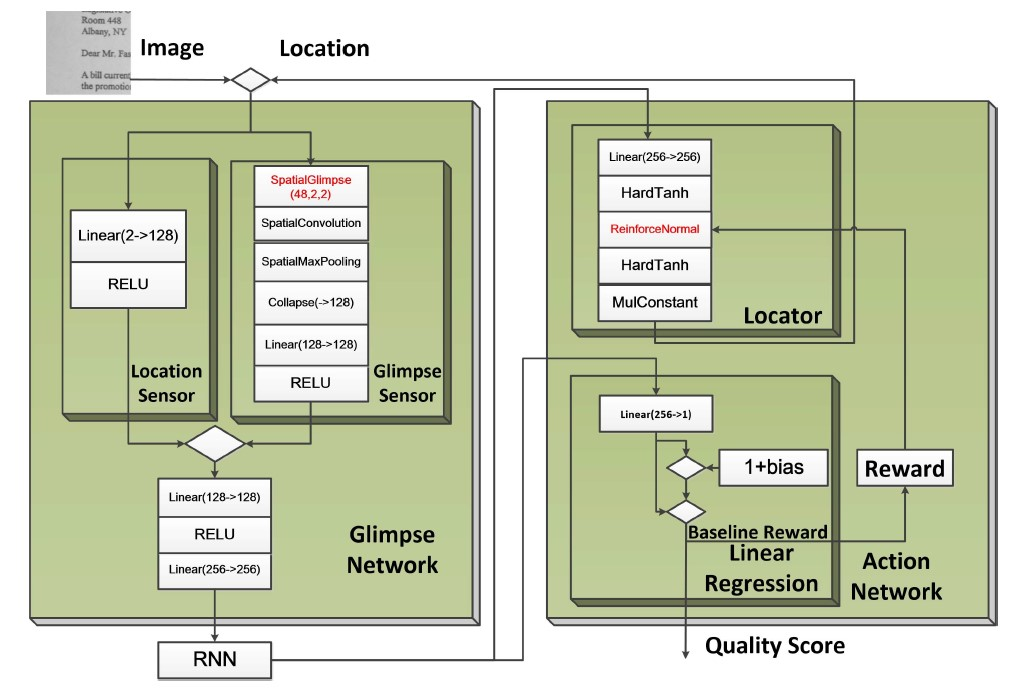
\includegraphics[width=0.6\textwidth]{Figures/AT_Li.jpg}
    \caption[Architecture of Li's proposed network]{Architecture of Li's proposed network}\cite{liAttentionBasedRNN2017}
    \label{fig:Li's Proposed Architecture}
\end{figure}

RNNs are good at handling sequential information but are poor at handling spatial information. CRNN's are more complex and combine the strengths of CNNs and RNNs which is more suitable for the this paper's OCR task.



\newpage

\subsection{Rule-based systems}

These were some of the earliest methods for OCR and use specific rules for identifying characters based on their shape, size, and relative position. They are now less commonly used due to their limitations with complex and diverse inputs.

Doush et al.'s paper "A novel Arabic OCR post-processing using rule-based and word context techniques" developed a rule-based OCR system for Arabic text that uses a combination of horizontal and vertical projections to segment characters and then classifies them based on their shape and relative position. \cite{doushNovelArabicOCR2018}



\begin{figure}[ht]
    \centering
    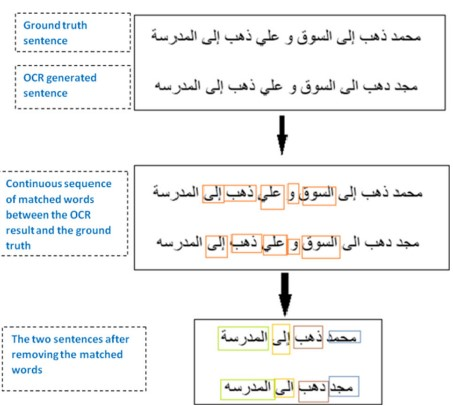
\includegraphics[width=0.6\textwidth]{Figures/RB_Doush.jpg}
    \caption[Example of applying the Rule Based FAHTA Algorithm]{Example of applying the Rule Based FAHTA Algorithm}\cite{doushNovelArabicOCR2018}
    \label{fig:Doush Rule Based OCR Paper}
\end{figure}

The FAHTA algorithm is a novel alignment technique that is used to match the ground truth text with the OCR misrecognized text. The paper also says that the FAHTA algorithm is fast, accurate, and can handle different types of OCR errors, such as over-segmentation, under-segmentation, and merging words. The paper claims that the FAHTA algorithm can be used for other languages as well.


For the purposes of this project, the rule-based system is not suitable because it requires a large number of rules to be defined for each character, which is not feasible for the large range of digit fonts.


\newpage

\subsection{Support Vector Machines (SVMs)}

Support Vector Machines (SVMs) are used for character recognition in OCR due to their effective high-dimensional mapping and classification abilities. They work best when text is clearly segmented. In the their paper "Development of an Image Processing Techniques for Vehicle Classification Using OCR and SVM", Joshua et al. used SVMs to classify characters in a license plate image and achieved an accuracy of 98.3\% using a local dataset of 10,000 images.\cite{joshuaDevelopmentImageProcessing2023}

\begin{figure}[ht]
    \centering
    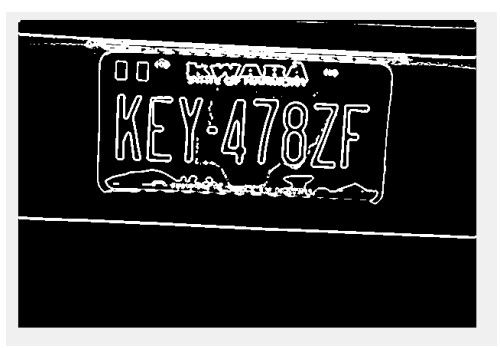
\includegraphics[width=0.8\textwidth]{Figures/SVM_Joshua.jpg}
    \caption[Development of an Image Processing Technique for Vehicle Classification using OCR and SVM]{Greyscale image with background cleaning}\cite{joshuaDevelopmentImageProcessing2023}
    \label{fig:Joshua SVM Paper}
\end{figure}

Joshua et al. describe the steps of their proposed system, which include image pre-processing, feature extraction, OCR, and SVM classification. They also explain how they collected and labelled their dataset of Nigerian vehicle plate numbers.

\newpage

\subsection{Hidden Markov Models (HMMs)}

HMMs have been used in OCR for recognizing sequential data. HMMs are statistical models that assume an underlying process to be a Markov process with hidden states.


In Rashid et al.'s "An evaluation of HMM-based Techniques for the Recognition of Screen Rendered Text" paper, they evaluate Hidden Markov Model (HMM) techniques for optical character recognition (OCR) of low resolution text from screen images and compares them with other OCR systems.

The paper uses two data sets of screen rendered characters and text-lines, and extracts two types of features from them: grey scale raw pixel features and gradient based grey level intensity features.


\begin{figure}[!h]
    \centering
    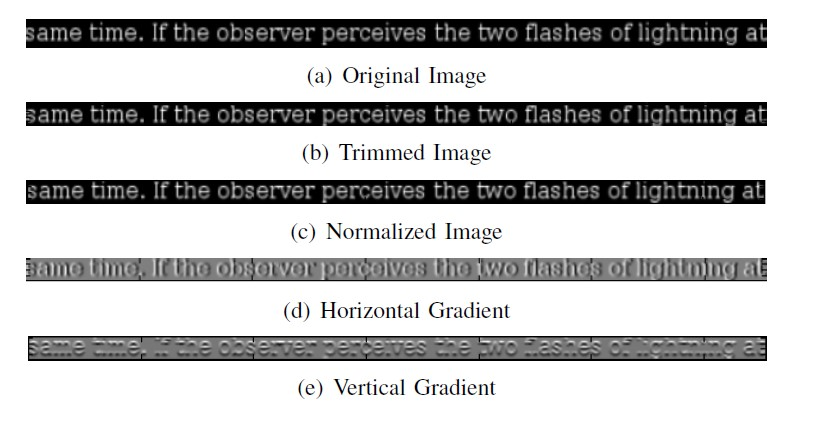
\includegraphics[width=0.8\textwidth]{Figures/HMM_Rashid.jpg}
    \caption[Rashid's Extraction steps from screen rendered text-lines]{Rashid's Extraction steps from screen rendered text-lines}\cite{rashidEvaluationHMMBasedTechniques2011}
    \label{fig:Rashid Feature Extraction Steps}
\end{figure}

The paper reports the character recognition accuracy of the HMM-based methods and other OCR engines on the two data sets. It shows that the HMM-based methods reach the performance of other methods on screen rendered text and achieve above 98\% accuracy.\cite{rashidEvaluationHMMBasedTechniques2011}

HMMs are a good choice for tasks where simplicity and interpretability are important. CRNNs are a good choice for tasks where accuracy is more important, and where the sequences are long or complex.

\newpage

\subsection{K-Nearest Neighbours (KNN)}

KNN is a simple, instance-based learning algorithm used for OCR, particularly for isolated character recognition. Hazra et al. develop an optical character recognition (OCR) system that uses a custom image to train a k-nearest neighbour (KNN) classifier. They claim that their system can recognize handwritten or printed text in any language by changing the training image and labels. \cite{hazraOpticalCharacterRecognition2017}

\begin{figure}[!h]
    \centering
    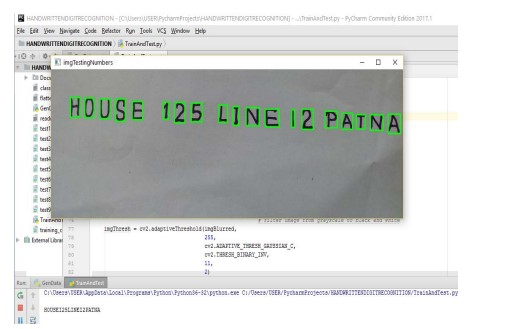
\includegraphics[width=0.8\textwidth]{Figures/KNN_Hazra.jpg}
    \caption[Optical Character Recognition using KNN on Custom
        Image Dataset]{Characters and Digits recognised}\cite{joshuaDevelopmentImageProcessing2023}
    \label{fig:Hazra OCR KNN Paper}
\end{figure}

Hazra et al. explain the steps of their algorithm, which include image processing, feature extraction, and KNN classification. They also discuss the advantages of KNN over other classification methods, such as ease of interpretation, low computation time, and high predictive power. In this paper the authors started with clear images of known fonts, which is not the case in this project.


\newpage

\subsection{Template Matching}

Template Matching is a technique used to locate small-parts of the bigger image which match a template image. This can be useful in OCR when the set of possible characters is known and limited. In Hossain et al.'s "Optical Character Recognition based on Template Matching" paper, they use template matching to recognize characters in a license plate image.

\begin{figure}[ht]
    \centering
    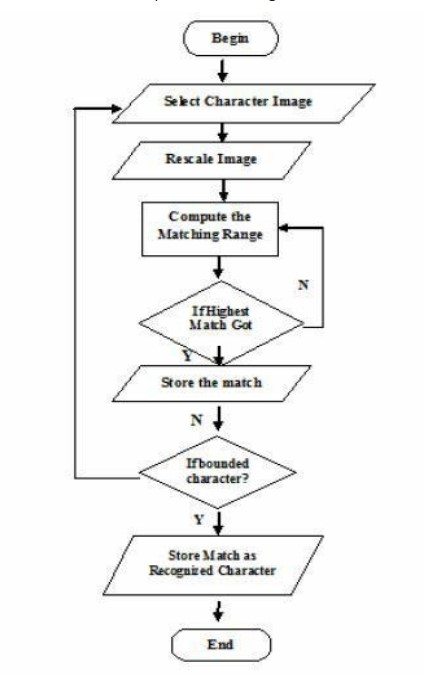
\includegraphics[width=0.4\textwidth]{Figures/TM_Hossain.jpg}
    \caption[Flowchart of Template Matching OCR]{Flowchart of Hossain's TM OCR}\cite{hossainOpticalCharacterRecognition2019}
    \label{fig:Hossain OCR Template Matching Paper}
\end{figure}

Their system prototype was tested on different text images with different fonts and sizes. The accuracy was calculated based on the character recognition accuracy. Their results show that Calibri and Verdana fonts had the highest accuracy, while Cambria and Times New Roman fonts had the lowest accuracy.  The accuracy can be improved by training the system with more fonts and features. \cite{hossainOpticalCharacterRecognition2019}

\newpage
\section{Conclusion}

Tesseract is an open-source optical character recognition (OCR) engine with a wide range of capabilities. It has been used to digitize ancient Tamil inscriptions, identify vehicles and their license plates, and recognize serial numbers on wine labels.

In this chapter, we have explored the capabilities and applications of Tesseract. We have seen that Tesseract can be used as a stand-alone tool, but it can also be combined with other technologies to improve its performance. For example, Tesseract can be integrated with object detection models to improve its accuracy at reading odometer mileage from car dashboard images.

We have also seen that Tesseract can be used in a variety of domains. For example, it has been used to preserve historical documents, aid linguistic research, and locate specific vehicles.

Overall, the potential of Tesseract OCR is vast. Its performance can be improved through integration with other models or pre-processing steps, and its applications extend to a variety of domains. The challenge lies in further refining the OCR technology, continuing to expand its range of uses, and exploring its potential for even more innovative applications in our increasingly digitized world.

Convolutional recurrent neural networks (CRNNs) are a powerful tool for processing sequential data and extracting important features. They have been shown to be effective in a variety of tasks, including optical character recognition (OCR), natural language processing, and image recognition.

CRNNs are able to handle variable-length sequential data and recognize long-term dependencies. This makes them ideal for tasks that require understanding of contextual and temporal information. For example, CRNNs can be used to recognize text in images, even if the text is of different languages or handwriting styles.

There have been many recent advances in CRNN research. For example, Biro et al. developed a CRNN that can recognize multilingual and hybrid language texts in OCR. Shinde et al. used CRNNs to recognize handwriting on forms, and Feng et al. used CRNNs to recognize container numbers.

These are just a few examples of the many applications of CRNNs. As research in this area continues, we can expect to see even more powerful and efficient CRNN models being developed. These models will have a wide range of applications, and will help us to better understand the world around us.